
O principal objetivo dos cenários de teste é apoiar a observação e a análise sistemática da técnica de auto-localização utilizada durante o trabalho, assim como as diferentes configurações do ambiente e
do filtro utilizado.

Após a realização de todos os cenários de teste propostos, foi possível chegar a uma conclusão quanto à viabilidade da utilização da técnica do Filtro de Partículas em um contexto típico da Robótica Educacional, a qual
será apresentada na seção \ref{sec:viabilidade}.

Os cenários de teste consistem em cinco situações, nas quais a solução foi analisada, variando entre elas o ambiente e a configuração do filtro. Buscando
analisar a exatidão da auto-localização obtida em cada contexto, reiterando que o objetivo da pesquisa é analisar a viabilidade da utilização
de uma técnica de SLAM em um contexto típico da Robótica Educacional.

O Filtro de Partículas é uma das duas principais técnicas que buscam solucionar o problema
de SLAM. Por este motivo, os cenários de teste desta pesquisa buscam analisar o Filtro de Partículas, sendo esse executado no contexto da Robótica Educacional.
A intenção é viabilizar, em parte, a aplicação da solução de SLAM nesse contexto.

Os dados obtidos a partir de cada cenário de teste está organizado de acordo com a Tabela \ref{tab:org_dados}.

\begin{table}[H]
  \centering
  \caption{Organização dos Dados}
  \label{tab:org_dados}
  \begin{tabular}{|c|c|c|c|c|c|}
  \hline
  \textbf{Ex.} & \textbf{Partículas} & \textbf{Rotação} & \textbf{Deslocamento} & \textbf{Ciclos} & \textbf{Precisão} \\ \hline
  \end{tabular}
\end{table}

Onde,
\begin{itemize}
  \item \textbf{Ex.} faz referência ao ciclo de teste. Cada cenário foi testado 5 (cinco) vezes, buscando obter a média como resultado
  final do cenário;

  \item \textbf{Partículas} informa a quantidade de partículas utilizada durante este teste;

  \item \textbf{Rotação} informa a velocidade de rotação do robô, em graus por segundo;

  \item \textbf{Deslocamento} informa a velocidade de deslocamento em linha reta, em centímetros por segundo;

  \item \textbf{Ciclos} apresenta o número de ciclos de filtragem que foram necessários para obtenção da localização;

  \item \textbf{Posição} informando qual a posição estimada do robô, informando a margem de erro da posição estimada, tanto no eixo X
  quanto no eixo Y. Basicamente, este campo informa de que ponto a que ponto nos eixos X e Y, o robô pode estar localizado, utilizando o
  centímetro como unidade, seguindo o padrão do restante da pesquisa.

  \item \textbf{Precisão} informando qual a precisão obtida no teste, classificada em \textit{Ótima}, \textit{Boa}, \textit{Mediana},
  \textit{Baixa} e \textit{Baixíssima}. A classificação da precisão é feita a partir da comparação entre a posição estimada e a posição real.
  Como a posição estimada possui uma margem de erro, destacada como uma elipse no local indicado, a comparação utiliza como referência
  esta elipse, assim como a partícula definida como sendo a que possui os dados mais próximos aos obtidos pelo robô real. A classificação
  segue a tabela \ref{tab:class_precisao}.

  \begin{table}[H]
    \centering
    \caption{Classificação da Precisão.}
    \label{tab:class_precisao}
    \begin{tabular}{|c|c|}
    \hline
    \textbf{Precisão} & \textbf{Descrição}                                                                                                                                                                \\ \hline
    Ótima             & \begin{tabular}[c]{@{}c@{}}Posição real se encontra a menos \\ de 5 centímetros da partícula final.\end{tabular}                                                                  \\ \hline
    Boa               & \begin{tabular}[c]{@{}c@{}}Posição real se encontra a uma distância entre\\ 6 e 10 centímetros da partícula real, se encontrando,\\ ainda, dentro da elipse de erro.\end{tabular} \\ \hline
    Mediana           & \begin{tabular}[c]{@{}c@{}}Posição real se encontra próxima as fronteiras da\\ elipse de erro, com mais de 10 centímetros de distância\\ da partícula final.\end{tabular}         \\ \hline
    Baixa             & \begin{tabular}[c]{@{}c@{}}Posição real se encontra fora da elipse de erro, porém\\ a até 10 centímetros de distância da sua fronteira.\end{tabular}                              \\ \hline
    Baixíssima        & \begin{tabular}[c]{@{}c@{}}Posição real se encontra fora da elipse de erro, a uma\\ distância de mais de 10 centímetros da fronteira da elipse.\end{tabular}                      \\ \hline
    \end{tabular}
  \end{table}

\end{itemize}

Durante os quatro primeiros cenários de teste, o ambiente utilizado foi o apresentado na Figura \ref{img:map1}, na qual todos os
valores se encontram em centímetros (cm). O quinto cenário, \ref{sub:cen5}, utilizou um ambiente sem características específicas, como o apresentado
na Figura \ref{img:mapa_quadrado}, buscando analisar o comportamento do algorítmo em mapas quadrados ou retangulares.

\begin{figure}[H]
	\centering
	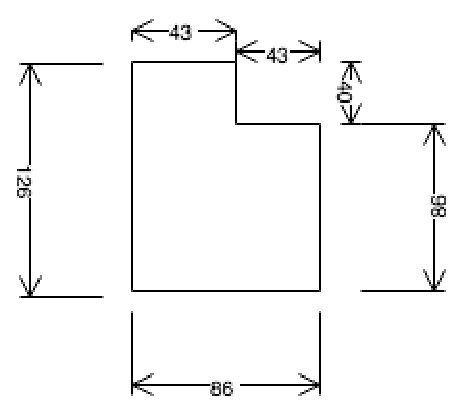
\includegraphics[scale=1.3]{figuras/map1.eps}
	\caption[Primeiro Cenário de Teste]{Mapa utilizado durante primeiro cenário de teste.}
	\label{img:map1}
\end{figure}

%Figura mapa quadrado aqui

Cada cenário de teste tem como objetivo observar o comportamento do Filtro de Partículas, levando em consideração o erro obtido
durante o processo de auto-localização. A variação entre cada cenário se dá pela alteração de três variáveis do processo de auto-localização:

\begin{itemize}
  \item Quantidade de partículas:

    Como o contexto trabalhado envolve recursos de \textit{hardware} limitados, o buscou-se selecionar uma quantidade relativamente
    baixa de partículas para execução do filtro, garantindo uma a ausência de grandes "furos" no mapa. A partir da execução do primeiro
    cenário de teste, com resultados disponíveis na Tabela \ref{tab:cen1}, foi fixado o valor de 150 (cento e cinquenta) partículas
    distribuídas aleatoriamente pelo mapa.

    Esta escolha se deu a partir de análise empírica, utilizando como parâmetros comparativos o processamento necessário para execução
    do Filtro de Partículas, a uniformidade da distribuição das partículas pelo mapa, a quantidade de ciclos necessários para conclusão
    da posição atual do robô e o erro final do processo.

  \item Velocidade de Rotação

    A seção \ref{sec:fontes_de_erros} apresenta como uma das principais fontes de erros o deslize entre a roda e o piso ao se movimentar.
    Desse modo, a escolha da velocidade se deu, principalmente, buscando minimizar o erro final. A velocidade de rotação foi fixada,
    a partir do cenário \ref{sub:cen3} no valor de 30 graus por segundo, a qual apresentou o menor erro final nos cenários anteriores.

  \item Velocidade de Deslocamento

    Assim como o parâmetro discutido anteriormente, este envolve a potencialização de uma fonte de erros para o processo
    de auto-localização, o deslize entre as rodas e o piso, como é apresentado na seção \ref{sec:fontes_de_erros}. O valor deste parâmetro
    não foi fixado durante os cenários com o mapa \ref{img:map1}, foi apenas reutilizado o valor de 30 diâmetros de roda por segundo,
    o que significa forçar a maior velocidade do robô.

    Utilizar a maior velocidade possível se torna possível devido a estratégia utilizada para minimizar esta fonte de erro, como é
    apresentado na seção \ref{sec:fontes_de_erros}.


  Estas informações podem ser obtidas na seção \ref{sub:cen1} e no apendice \ref{sec:dados_cenarios_teste}.
\end{itemize}

As seções \ref{sub:cen1}, \ref{sub:cen2}, \ref{sub:cen3}, \ref{sub:cen4} e \ref{sub:cen5} apresentam os cenários de teste com a variação dos parâmetros, possibilitando a análise do comportamento do robô
com determinadas configurações de parâmetros.

\subsection{Cenário de Teste 1}
\label{sub:cen1}

Os resultados obtidos com o cenário estão dispostos na Tabela \ref{tab:cen1}. Deve-se atentar que o exemplo 3 possui um agravante, o
robô teve sua roda direita presa na parede, enquanto se locomovia. Desse modo, o robô perdeu-se e teve que se encontrar novamente, comportando-se
da maneira esperada em um caso básico de "sequestro do robô".

Este cenário faz referência à variação da quantidade de partículas.

\begin{table}[H]
\centering
\caption{Resultados Obtidos - Cenário 1}
\label{tab:cen1}
\begin{tabular}{|c|c|c|c|c|c|c|}
\hline
\textbf{Ex.} & \textbf{Partículas} & \textbf{Rotação} & \textbf{Deslocamento} & \textbf{Ciclos} & \textbf{Posição}                                            & \textbf{Precisão} \\ \hline
1                & 200                 & 100              & 100                   & 9                   & \begin{tabular}[c]{@{}c@{}}X: 25 a 70\\ Y: 15 a 30\end{tabular} & Ótima             \\ \hline
2                & 400                 & 100              & 100                   & 10                  & \begin{tabular}[c]{@{}c@{}}X: 17 a 37\\ Y: 39 a 66\end{tabular} & Boa               \\ \hline
3                & 500                 & 100              & 100                   & 21                  & \begin{tabular}[c]{@{}c@{}}X: 35 a 54\\ Y: 34 a 82\end{tabular} & Mediana           \\ \hline
4                & 100                 & 100              & 100                   & 5                   & \begin{tabular}[c]{@{}c@{}}X: 50 a 63\\ Y: 39 a 69\end{tabular} & Mediana           \\ \hline
5                & 150                 & 100              & 100                   & 3                   & \begin{tabular}[c]{@{}c@{}}X: 74 a 76\\ Y: 66 a 69\end{tabular} & Ótima             \\ \hline
\end{tabular}
\end{table}

A partir da análise empírica deste cenário de teste, foi possível identificar que o número de partículas necessárias para realização, com
qualidade, do processo de auto-localização seria de 150 partículas. Isto se dá devido à relação entre o processamento necessário para execução
do filtro e a uniformidade da distribuição das partículas pelo mapa.

A partir do cenário \ref{sec:cen2}, a quantidade de partículas utilizadas foi fixada em 150 partículas, devido ao apresentado anteriormente.
Os dados que levaram a esta escolha podem ser observados em \ref{sec:cenario1}.

\subsection{Cenário de Teste 2}
\label{sub:cen2}

Os resultados obtidos com o cenário estão dispostos na Tabela \ref{tab:cen2}. Este cenário faz referência à variação da velocidade de
rotação do robô, a qual é mensurada em graus por segundo.

\begin{table}[H]
\centering
\caption{Resultados Obtidos - Cenário 2}
\label{tab:cen2}
\begin{tabular}{|c|c|c|c|c|c|c|}
\hline
\textbf{Ex.} & \textbf{Partículas} & \textbf{Rotação} & \textbf{Deslocamento} & \textbf{Ciclos} & \textbf{Posição}                                            & \textbf{Precisão} \\ \hline
1                & 150                 & 10               & 100                   & 7                   & \begin{tabular}[c]{@{}c@{}}X: 30 a 72\\ Y: 47 a 71\end{tabular} & Boa               \\ \hline
2                & 150                 & 30               & 100                   & 6                   & \begin{tabular}[c]{@{}c@{}}X: 20 a 38\\ Y: 42 a 67\end{tabular} & Ótima             \\ \hline
3                & 150                 & 50               & 100                   & 3                   & \begin{tabular}[c]{@{}c@{}}X: 29 a 63\\ Y: 30 a 62\end{tabular} & Boa               \\ \hline
4                & 150                 & 70               & 100                   & 3                   & \begin{tabular}[c]{@{}c@{}}X: 23 a 66\\ Y: 29 a 68\end{tabular} & Mediana           \\ \hline
5                & 150                 & 90               & 100                   & 8                   & \begin{tabular}[c]{@{}c@{}}X: 36 a 61\\ Y: 15 a 35\end{tabular} & Mediana           \\ \hline
\end{tabular}
\end{table}

A partir da análise empírica destes resultados, fixou-se o valor da velocidade de rotação em 30 graus por segundo. Esta definição
se deu devido a comparação dos resultados obtidos, utilizando o erro final como variável comparativa. Desse modo, a partir do cenário
\ref{sub:cen3}, a velocidade de rotação foi fixada no valor de 30 graus por segundo.

Estes registros podem ser visualizados na seção \ref{sec:cenario2}.


\subsection{Cenário de Teste 3}
\label{sub:cen3}

Os resultados obtidos com o cenário estão dispostos na Tabela \ref{tab:cen3}. Este cenário faz referência à variação da velocidade de
deslocamento do robô, em unidades do diâmetro das rodas por segundo.

\begin{table}[H]
\centering
\caption{Resultados Obtidos - Cenário 3}
\label{tab:cen3}
\begin{tabular}{|c|c|c|c|c|c|c|}
\hline
\textbf{Ex.} & \textbf{Partículas} & \textbf{Rotação} & \textbf{Deslocamento} & \textbf{Ciclos} & \textbf{Posição}                                            & \textbf{Precisão} \\ \hline
1                & 150                 & 30               & 2                     & 4                   & \begin{tabular}[c]{@{}c@{}}X: 30 a 70\\ Y: 28 a 62\end{tabular} & Baixa             \\ \hline
2                & 150                 & 30               & 5                     & 6                   & \begin{tabular}[c]{@{}c@{}}X: 31 a 59\\ Y: 32 a 70\end{tabular} & Mediana           \\ \hline
3                & 150                 & 30               & 10                    & 3                   & \begin{tabular}[c]{@{}c@{}}X: 30 a 73\\ Y: 20 a 78\end{tabular} & Baixa             \\ \hline
4                & 150                 & 30               & 15                    & 6                   & \begin{tabular}[c]{@{}c@{}}X: 82 a 89\\ Y: 73 a 82\end{tabular} & Boa               \\ \hline
5                & 150                 & 30               & 30                    & 5                   & \begin{tabular}[c]{@{}c@{}}X: 23 a 54\\ Y: 40 a 73\end{tabular} & Mediana           \\ \hline
\end{tabular}
\end{table}

Durante a execução dos exemplos dispostos na Tabela \ref{tab:cen3}, foi possível identificar uma solução simples para a fonte de erro
\ref{sub:deslizes}, a qual possibilitou a fixação da velocidade como 15 diâmetros por segundo. Este valor significa, assim como o valor de 30 diâmetros por segundo, a máxima
velocidade do kit, dado que é um valocidade inalcançável, por parte do kit Mindstorm NXT.

Esta solução envolve, como é descrito na seção \ref{sec:fontes_de_erros}, a utilização de um processo de aceleração, até alcançar a velocidade
definida. Desse modo, foi possível obter melhores resultados durante o processo de auto-localização, de acordo com análises empíricas do
processo como um todo.

\subsection{Cenário de Teste 4}
\label{sub:cen4}

Os resultados obtidos com o cenário estão dispostos na Tabela \ref{tab:cen4}. Este cenário faz referência à análise da solução
utilizando a configuração que obteve os melhores resultados nos cenários anteriores, ou seja:

\begin{itemize}
  \item \textbf{Partículas:} 150
  \item \textbf{Rotação:} 30 graus por segundo
  \item \textbf{Deslocamento:} 15 diâmetros por segundo (velocidade máxima)
\end{itemize}

O objetivo principal deste cenário é verificar a variabilidade dos resultados utilizando configuração fixa durante os exemplos.

\begin{table}[H]
\centering
\caption{Resultados Obtidos - Cenário 4}
\label{tab:cen4}
\begin{tabular}{|c|c|c|c|c|c|c|}
\hline
\textbf{Ex.} & \textbf{Partículas} & \textbf{Rotação} & \textbf{Deslocamento} & \textbf{Ciclos} & \textbf{Posição}                                            & \textbf{Precisão} \\ \hline
1                & 150                 & 30               & 15                    & 8                   & \begin{tabular}[c]{@{}c@{}}X: 30 a 54\\ Y: 28 a 45\end{tabular} & Mediana           \\ \hline
2                & 150                 & 30               & 15                    & 4                   & \begin{tabular}[c]{@{}c@{}}X: 62 a 87\\ Y: 23 a 58\end{tabular} & Baixa             \\ \hline
3                & 150                 & 30               & 15                    & 5                   & \begin{tabular}[c]{@{}c@{}}X: 27 a 75\\ Y: 10 a 32\end{tabular} & Baixíssima        \\ \hline
4                & 150                 & 30               & 15                    & 7                   & \begin{tabular}[c]{@{}c@{}}X: 66 a 70\\ Y: 27 a 33\end{tabular} & Mediana           \\ \hline
5                & 150                 & 30               & 15                    & 8                   & \begin{tabular}[c]{@{}c@{}}X: 37 a 67\\ Y: 34 a 67\end{tabular} & Boa               \\ \hline
\end{tabular}
\end{table}

O cenário de teste \ref{sub:cen5} apresenta o processo de auto-localização em um mapa retangular, buscando analisar o comportamento do
algoritmo em um ambiente com referenciais de baixa unicidade.

\subsection{Cenário de Teste 5}
\label{sub:cen5}

Os resultados obtidos com o cenário estão dispostos na Tabela \ref{tab:cen5}.

\begin{itemize}
  \item \textbf{Partículas:} 150
  \item \textbf{Rotação:} 30
  \item \textbf{Deslocamento:} 15
\end{itemize}

O objetivo deste cenário é verificar a viabilidade da utilização do Filtro de Partículas em um ambiente sem pontos de referência únicos.

\begin{table}[H]
\centering
\caption{Resultados Obtidos - Cenário 5}
\label{tab:cen5}
\begin{tabular}{|c|c|c|c|c|c|c|}
\hline
\textbf{Ex.} & \textbf{Partículas} & \textbf{Rotação} & \textbf{Deslocamento} & \textbf{Ciclos} & \textbf{Posição}                                            & \textbf{Precisão} \\ \hline
1                & 150                 & 30               & 15                    & 6                   & \begin{tabular}[c]{@{}c@{}}X: 21 a 63\\ Y: 40 a 84\end{tabular} & Mediana           \\ \hline
2                & 150                 & 30               & 15                    & 11                   & \begin{tabular}[c]{@{}c@{}}X: 37 a 70\\ Y: 47 a 90\end{tabular} & Mediana             \\ \hline
3                & 150                 & 30               & 15                    & 6                   & \begin{tabular}[c]{@{}c@{}}X: 27 a 75\\ Y: 10 a 32\end{tabular} & Mediana        \\ \hline
4                & 150                 & 30               & 15                    & 7                   & \begin{tabular}[c]{@{}c@{}}X: 66 a 70\\ Y: 27 a 33\end{tabular} & Mediana           \\ \hline
5                & 150                 & 30               & 15                    & 11                   & \begin{tabular}[c]{@{}c@{}}X: 37 a 67\\ Y: 34 a 67\end{tabular} & Mediana               \\ \hline
\end{tabular}
\end{table}

De acordo com o resultado obtido durante a execução dos exemplos apresentados na Tabela \ref{tab:cen5}, a qual possui seus registros
dispostos na seção \ref{sec:cenario5}, o robô é capaz de se alto-localizar no ambiente retangular. A análise deste resultado se encontra
na seção \ref{sec:viabilidade}.

A partir da observação e análise empírica durante a realização dos cenários apresentados anteriormente, foi possível identificar
fontes específicas de erros. Assim como obter uma conclusão sobre a viabilidade da resolução parcial do problema de SLAM em um contexto
limitado da Robótica Educacional. As seções \ref{sec:fontes_de_erros} e \ref{sec:viabilidade} registram estes resultados obtidos durante
a pesquisa.
